\chapter{FANET routing protocol}
Each multi-UAV mission has its own set of requirements in terms of size and number of vehicles, the size of the mission's region, payload, mission duration, environmental constraints, level of autonomy and mobility requirements. These all mission-oriented requirements - in turn - generate a peculiar set of demands from the communication infrastructure. Therefore, we will first present an overview of our multi-UAV mission at hand, the communication requirements and then a protocol that facilitates those primitives.

\section{FANET Mission}

The use of multi-cluster UAVs to track gas plumes like volcanic eruptions, forest fires, and environmental contamination has increased in the previous decade. The network requirement from a FANET depends on the mission. For example, in a plume tracking mission, the UAVs would be required to wrap around the plume, report the contamination level and possibly move with the plume. Once the UAVs have been deployed they have complete device autonomy (i.e. each UAV decides its future waypoints and velocity itself using the inputs of onboard sensors and don't need these instructions from a human operator) and mission autonomy (i.e. the UAVs must cooperate and coordinate with each other for the successful completion of the mission). It should also be noted that although the UAVs coordinate in the decision-making process, a network-wide consensus is not required for a specific UAVs operation. As the plume moves in time and space the UAVs should evenly spread out on the surface of the plume while maintaining a safe distance from each other and avoiding any static or dynamic obstacle in their path. 

A detailed description of the problem and a multi-UAV distributed solution has been provided in \cite{8080382}. In the proposed solution the authors have assumed that the mission starts with an initial formation of drones in a 2-dimensional grid (shown in \fref{fig:mesh_formation}). Thereafter, the UAVs move towards the plume autonomously without any ground support. Whenever a UAV detects a contamination it stops and maintains its position with respect to the plume while rest of the UAVs continue their search. If the inter-UAV distance crosses a threshold (too close or too far away) then the moving drone tries to move further or closer to the stationary UAV. These inter-drone forces maintain an approximate mesh structure while resulting in the UAVs wrapping around the plume. As an aid to visualizing this process, think of the mesh as a piece of cloth moving towards a spherical ball and eventually wrapping around the ball. \fref{YYY} shows an intermediate state with drones wrapping around the plume and \fref{fig:final_state} shows a desired final state of UAVs wrapped around the plume.
  

\begin{figure}[hbtp]
\centering
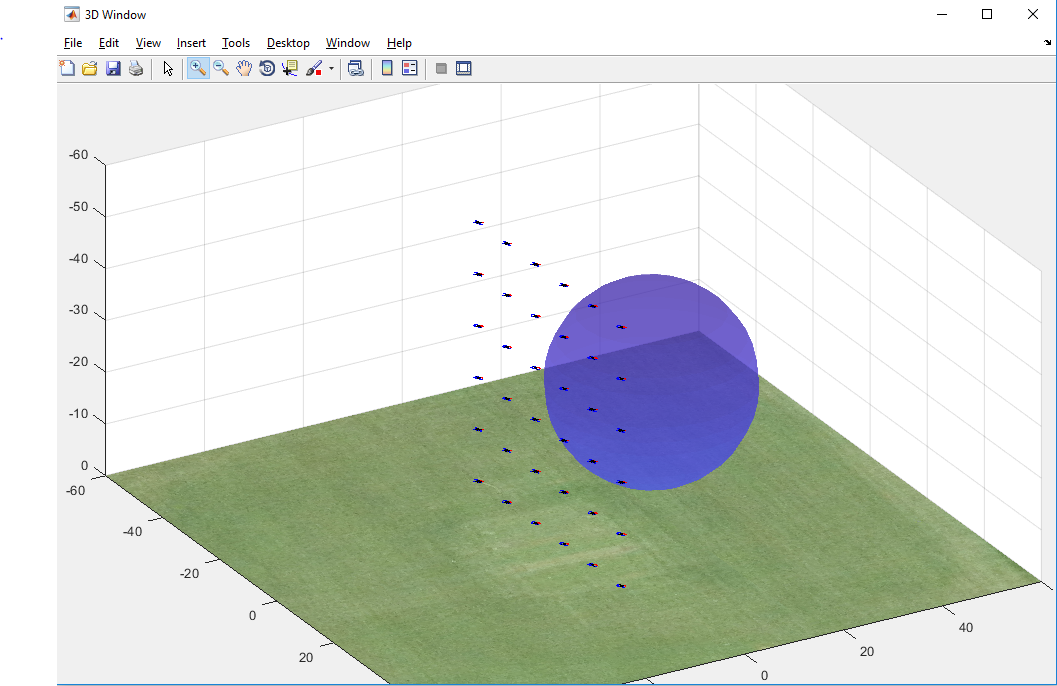
\includegraphics[width=0.8\textwidth]{Chapter-3/figs/initial_drone_config}
\caption{Mesh formation of UAVs at the start of the mission}
\label{fig:mesh_formation}
\end{figure}

\begin{figure}[hbtp]
\centering
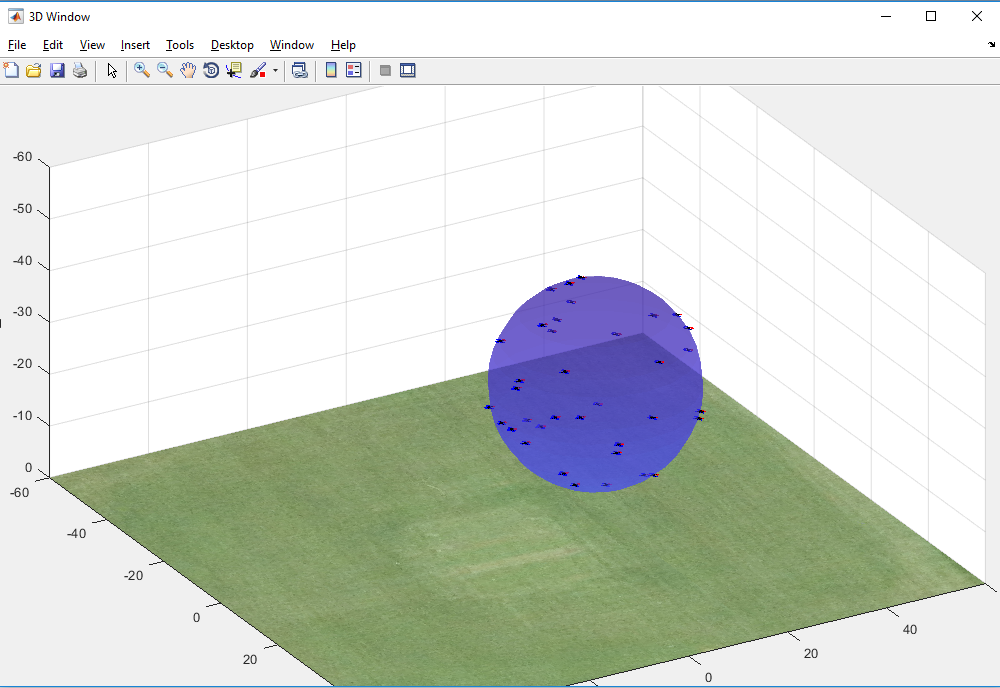
\includegraphics[width=0.8\textwidth]{Chapter-3/figs/final_formation}
\caption{Desired final state of UAVs wrapped around the plume}
\label{fig:final_state}
\end{figure}


\section{Communication requirements} \label{comm_reqs}
\textbf{Content}: There are different network requirements for communicating telemetry/ coordination and sensed data, some of them are delay tolerant and some need to be delivered to a specific region.

\textbf{Intent}: Discuss the scenarios where uav-to-uav, uav-to-ground station unicast would be required and the scenarios where geocast would be suitable. 

In this section, we shall outline the qualitative and quantitative requirements from a communications viewpoint for the successful communication of the mission. We shall use these requirements to design the routing protocol, the message primitives and eventually as a yardstick to measure the performance of the proposed protocol. It should also be noted that the requirements are geared towards a specific mission and since the UAV applications are diverse, these communication demands, and requirements shall widely vary for different applications. For a comprehensive analysis of various civil UAV applications, we refer the readers to \cite{7463007}, where the authors have classified the civil applications of UAVs into four broad categories, namely, Search and Rescue, Area or Network Coverage, Construction, Delivery/transportation and presented the requirements from a communications viewpoint. 

\textbf{Mission coverage:} Applications like plume tracking, wildfire monitoring or plume wrapping typically span a medium to large sized area in the order of tens of kilometers \cite{7463007}. Furthermore, the aerial network should consider the coverage volume expansion or shrinkage with time. The mission volume that we shall be considering would be $ \approx 1500 m \times 1500 m \times 1000 m $. 

\textbf{Network requirement:} Since the mission requires coordination among the participating UAVs, any two participating UAVs should be able to reliably communicate with each other (either directly or multi-hop connectivity). Moreover, the network should be able to reconfigure itself, in other words, the network should consider the nodes joining and leaving the network while the mission is in progress.

\textbf{Number of nodes:} The number of UAVs required in a mission depends on the mission area, transceiver characteristics and the type of nodes employed. Assuming off-the-shelf Wi-fi transceivers and the above mentioned mission coverage the required number of nodes would be around 30. 

\textbf{Connectivity to a base station:} In a real-life deployment scenario, the UAVs must be connected to a base station for safety and security purposes, although the data-rate requirement of the link can be mission specific. In our case, the UAVs need to send their telemetry information (GPS and IMU data) to the base station, however since the mission is fully autonomous with distributed decision-making capacity the entities don’t need to relay the coordination data to the base station. A frequency of 4-5 Hz or less is the standard for telemetry data exchange \cite{7463007}. 

\textbf{Connectivity between the other UAVs:} Since the UAVs are required to maintain an approximate mesh structure they need to approximate the distance with other drones. Therefore, the UAVs need to update each other of their GPS locations in real-time. A suitable frequency of this data exchange could be 4-5 Hz. Also, in real deployment scenarios, the UAV cluster can be composed of drones with varying capabilities (UAVs have different sensors) which demands a need for one-to-one communication. Therefore, the UAVs must have a reliable connectivity to each other in either a single or multi-hop fashion. 

\textbf{Traffic Demands:} The traffic in the aerial UAV network consists of control data (remote controlled data exchange), telemetry data (GPS and IMU data), coordination data (waypoint, mission plan exchange) and sensed data (sensor data). The actual traffic demands depend on the sensor-on-board the UAVs, the type of traffic exchanged in the network and the frequency of such exchange. As per \cite{NASA_UAV_mission_parameters}, imagery and chemical data would need to be collected which would require chemical analyzer, an infrared sensor, image or possibly a video camera. The sensed traffic is sensor dependent and can be, low-rate, bursty or high-rate. In our case, the UAVs need to exchange coordination data among each other, sensed data with the base station and telemetry data with each other as well as the base station. The data exchange with the base station can be periodic and delay-tolerant but the coordination data among the drones must real-time. As far as data rate is concerned 1 Mbps for images and 2 Mbps for video streaming is sufficient with a typical delay of not more thatn 50-100 ms \cite{7463007}. 

\textbf{Collision Avoidance:} Once a UAV detects another UAV (e.g. via RADAR) in its flight path, they both need to navigate around each other to avoid a collision. To check if a future waypoint is void of other UAVs, the source UAV can send an anycast to that specific destination region. If some other UAV happens to be in the region then they should negotiate their way around. It should be noted that the originator UAV doesn't know or care about the identity of the drone, rather the message is addressed to the geographical region. This requires a capability to geocast packets where the destination location is the address. These messages are not delay-tolerant and need to be delivered in real time.

\textbf{Scalability:} The number of nodes can be increased due to two reasons. (1) Increase the coverage volume (2) Increase the density of nodes to get a high-resolution sensory data. A scalabilable network  should handle the increase in a number of nodes/devices in the network and the performance should not degrade unreasonably. 

\textbf{Localization and time synchronization:} The UAVs need to know and report their own location with an accuracy of $\approx 5 m$. This level of accuracy is achievable with off-the-shelf GPS devices and can be improved to a few centimeters by using dual-frequency receivers and/or augmentation systems \cite{gps_accuracy} . The UAVs can also synchronize their clocks through the information provided by GPS.

The above information is summarized in table \ref{tab:communication_requirements}.
\begin{table}
\caption{Communication requirements}
\label{tab:communication_requirements}
\begin{tabular}{|p{0.38\linewidth}|p{0.47\linewidth}|}
\toprule
Requirements & Values\\
\midrule
Mission Coverage & Medium or Large $\approx 1500 m \times 1500 m \times 1200 m$ \\
\midrule
Network mode & ad hoc \\
\midrule
Number of nodes &  $\approx 30 $ \\
\midrule
Coordination data exchange frequency &  4-5 Hz \cite{7463007}\\
\midrule
Sensed data exchange frequency & 30 Hz for video, 1 Hz for IR and chemical analyzer \cite{7463007}\\
\midrule
Telemetry data exchange frequency & 4-5 Hz \cite{7463007}\\
\midrule
Coordination data link rate (up/down) & 4.8 /64 kbaud \cite{7463007} \\
\midrule
Sensed data link rate (up/down) & 4.8-9.6/64 kbaud \cite{NASA_UAV_mission_parameters} \\
\midrule
Delay & 50-100 ms \cite{7463007}\\
\midrule
Traffic type & periodic and real time (coordination data, telemetry data), delay tolerant (sensed data) \\
\bottomrule
\end{tabular}
\end{table}

\section{Routing protocol} \label{routing_protocol}

\textbf{Content: Discuss the location service employed to get destination location, packet header, message primitives and packet routing strategy.}

\textbf{Intent: Explain how a node knows the location of the destination node, and when a node transmits a received message.
}

In this section, we shall first discuss our underlying assumptions in presenting our routing scheme, the packet header and then we shall discuss the message primitives derived from the communication requirements presented in section \ref{comm_reqs}.  

\textbf{Assumptions:}
\begin{enumerate}
\item The wireless antennas on the nodes are omnidirectional.
\item The nodes are reachable from each other i.e. a flooding algorithm can guarantee packet delivery between any pair of nodes and we use the delivery rate of flooding algorithm as an upper bound for our algorithm.
\item The nodes always know their location via GPS. 
\item The nodes synchronize their clock via GPS.
\item A source node knows an approximate location of the destination node which is maintained in a location table and provided by a location service. Different implementations of a location service have been mentioned in section \ref{loc_service} and our implementation has been explained in section \ref{loc_service_impl}. 
\end{enumerate}

\subsection{Packet Header} \label{packet_header}
We first define the packet header that the source node attaches to the payload.
\begin{itemize}
\item Packet ID (\emph{pId}): A number that uniquely identifies this packet among those transmitted by this node. The combination of source node identification and packet ID should uniquely identify a packet in the FANET. 
\item Source Node ID (\emph{srcId}): A unique identifier for the source node. It could be IP address of the node.
\item Source Location (\emph{sLoc}): The GPS coordinate of the source node.
\item Destination Node ID (\emph{destId}): A unique identifier for the destination node. If a packet is destined to a geographical region, then this shall be set to the macro ANY. If a packet is to be flooded in the network, then this value should be set to the macro FLOOD. 
\item Destination Location (\emph{dLoc}): GPS coordinate of the destination as known to the source node. In case of flood packet, this would be set to NULL or be ignored. 
\item Radius (\emph{r}): In case of a geocast packet, the radius along with dLoc defines the destination spherical region for the packet.
\item Transmitter ID (\emph{trId}): A unique identifier for the latest transmitter of the packet.
\item Transmitter Location (\emph{trLoc}): GPS coordinate of the node that had last transmitted the packet.
\item Timestamp (\emph{timestamp}): The time when this packet was transmitted by the source.
\item Width (\emph{w}): The width of the transmission zone for the packet. Explained later in this section.
\item Hops To Live (\emph{HTL}): A node forwards a message only if HTL > 0 and reduces HTL by 1 before forwarding the packet. 
\item Acknowledgement Required (\emph{ackReq}): This flag denotes whether the source node is expecting an \emph{ack} reply.
\item Update Allowed (\emph{update}): This flag denotes whether an intermediate node can update the message headers. For example, if the intermediate node has a location update that is later than the message's \emph{timestamp}.

\end{itemize}

\subsection{Message primitives} \label{message_primitives}

As discussed in section \ref{comm_reqs} the following data exchange happen in the mission:
\begin{enumerate}
    \item UAV to all UAVs: Telemetry data (e.g. GPS, IMU data).
    \item UAV to base station: Telemetry data and sensed data.
    \item UAV to any UAV is a region: Coordination data (e.g. Future waypoint).
\end{enumerate}

To facilitate the above data exchange we should support the following message primitives:
\begin{enumerate}
\item \emph{Flood(message, sourceID)}
\item \emph{Unicast(message, sourceID, destinationID)}
\item \emph{Geocast(message, sourceID, destinationCoordinates, radius)}
\end{enumerate}

Here \emph{sourceID} and \emph{destinationID} are unique identifiers for a node - possibly IP addresses, while \emph{destinationCoordinates} together with \emph{radius} represent a spherical region with specified coordinate as the center and specified radius.

We will now present a high-level algorithmic description of these message primitives.

\paragraph{Flood}

Flood primitive is ensures that the packet shall be received by all the nodes that are connected. When a source node `S' needs to send a message to every node in the network, it creates a header with the following parameters and encapsulates the data in this header.

\begin{eqnarray*}
& header = & messageHeader(destId = FLOOD, dLoc = IGNORE, \\
&    & radius = IGNORE, pdate = IGNORE, width = IGNORE, \\
&    & ackReq = FALSE, HTL = NETWORK\textunderscore DIAMETER)
\end{eqnarray*} 

Node `S' then broadcasts this message to all its neighbors in the wireless medium. An intermediate node 'N', on receiving the message for the first time reads the contents and rebroadcasts it. Thereafter, `N' discards any duplicate receptions of the message. This guarantees that the flooding is loop-free. The benefit of Flooding is the protocol's robustness however there is a high overhead associated with flooding and hence it is suitable for small packets only.

The primitive allows to restrict the span of flooding by the HTL parameter. For example, if a source node `S' wants to send a message to all its immediate neighbors (i.e. in direct radio range) then `S' shall set the HTL value to 1 in the header.

The part of receive algorithm that deals with FLOOD packets is depicted in algorithm \ref{flood_recv}

\begin{algorithm}
\caption{Receive(msg): Flood} 
\label{flood_recv}
\DontPrintSemicolon
\SetKwProg{Receive}{Receive}{}{}
\Receive{(msg)}{%
    \If{msg.pId $\in$ transmittedMsgIdSet}{
        discard(msg)\;
        EXIT\;
    }
    \eIf {msg.destId == FLOOD}{
        \eIf{msg.pId $\notin$ seenIdSet} {
            msg.HTL = msg.HTL - 1\;
            Add (seenIdSet, msg.pId)\;
            \If {msg.HTL > 0}{
                transmit(msg)\;
            }
        }{
            discard(msg)\;
        }
    }{
    ...
    }
}

\end{algorithm}

\paragraph{Geocast}

Geocast is used when a UAV wants to communicate with any node present in a geographic region. This is useful in scenarios where two nodes with a conflicting path and need to communicate to negotiate the path. The underlying mechanism of geocast is flooding but we restrict the flooding to a specific `zone' i.e. if an intermediate node happens to be in that `zone' then only the intermediate node shall re-transmit that message.  

\begin{figure}[hbtp]
\centering
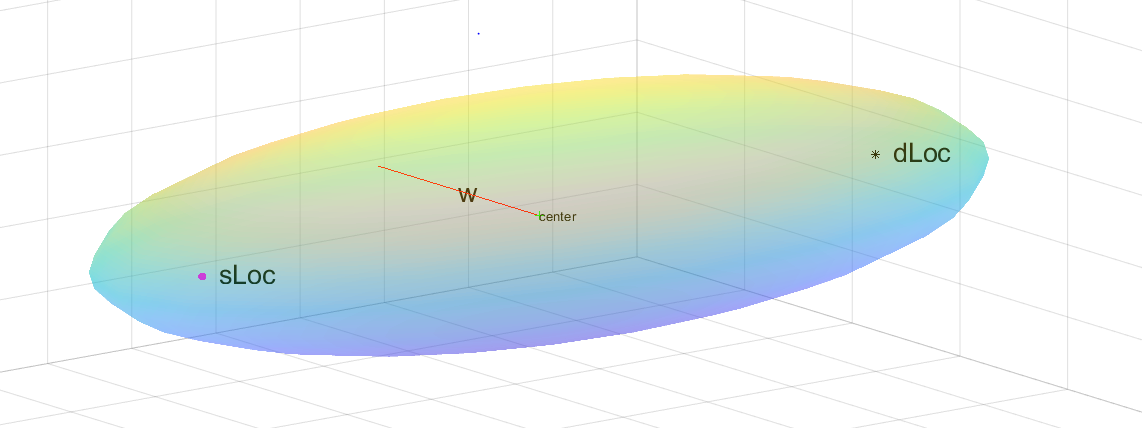
\includegraphics[width=1\textwidth]{Chapter-3/figs/Spheroid}
\caption{Transmission zone with source at sLoc and destination at dLoc}
\label{fig:spheroid}
\end{figure}

\textbf{Transmission Zone:} Consider source node `S' (at \emph{sLoc}) needs to send a message to a destination location \emph{dLoc}. The source node will first create a message (\emph{msg}) and defines a volume in the form of a spheroid with \emph{msg.sLoc} and \emph{msg.dLoc} as the two foci points and parameter \emph{msg.w} as the minor-axis length. An intermediate node `N' forwards this \emph{msg} if and only if `N' lies inside the spheroid defined by the \emph{msg} parameters. This idea of constrained flooding is derived from the concept of the petal in \cite{6133499} and that of request zone in \cite{Ko:1998:LRM:288235.288252}. To increase reliability, the source node can increase the parameter transmission zone's width \emph{msg.w}.

A sample depiction of transmission zone is depicted in \fref{fig:spheroid} where sLoc and dLoc are the foci points and `w' is the length of the minor axis.

When a source node `S' needs to send a message to \emph{any} node in a spherical region `R' with center at \emph{`dLoc'} and radius \emph{`r'} then `S' chooses an appropriate width `w' and creates a header with the following parameters.
\begin{eqnarray*}
& header = & messageHeader(destId = ANY, dLoc = [x,y,z], radius = r,\\
&    & update = IGNORE, width = w, ackReq = FALSE)
\end{eqnarray*}
Source node `S' then encapsulates the data in this header and transmits the packet. An intermediate node `N' processes the message according to the algorithm presented in \ref{geocast_recv}

\begin{algorithm}
\caption{Receive(msg): Geocast} 
\label{geocast_recv}
\DontPrintSemicolon
\SetKwProg{Receive}{Receive}{}{}

\Receive{(msg)}{
    \If{msg.pId $\in$ transmittedMsgIdSet}{
        discard(msg)\;
        EXIT\;
    }
    \If{msg.destId == ANY}{
        \If{insideDestinationRegion(msg, myLoc)}{
            Transmit(msg)\;
            Add msg.pId to transmittedMsgIdSet\;
            EXIT\;
        }
    }
    \If{insideTransmissionZone(msg, myLoc) == TRUE}{
        \eIf{msg.pId is in bufWait}{
            Increase duplicate count for msg.pId\; 
            save msg.tLoc\;
        }{
            boffTime = calculateBoffTime(msg)\;
            add msg to bufWait \;
            
            registerCallback(boffTime, msg)\;
        }
    }
}
\end{algorithm}

\paragraph{Unicast}

Unicast is used when a source node `s' needs to send a message to a destination node `D'. Unicast uses the same underlying mechanism as geocast to route a message except that `S' first consults its location table for `dLoc' - the location of destination `D' - and creates a header with the following parameters.

\begin{eqnarray*}
& header = & messageHeader(destId = destID, dLoc = dLoc,\\
&    & radius = IGNORE, update = IGNORE, width = w, \\
& & ackReq = FALSE)
\end{eqnarray*}

Source node `S' then encapsulates the data in this header and transmits the packet.
An intermediate receiving node `N' follows the algorithm \ref{unicast_recv}.

\begin{algorithm}
\caption{Receive(msg): Unicast} 
\label{unicast_recv}
\DontPrintSemicolon
\SetKwProg{Receive}{Receive}{}{}
\Receive{(msg)}{
    \If{msg.pId $\in$ transmittedMsgIdSet}{
        discard(msg)\;
        EXIT\;
    }
    \eIf{msg.destId = myId}{
        \If{msg.ackReq == TRUE}{
            ackRep = prepareAckReply()\;
            send(ackRep);
        } 
    }
    {
        algorithm \ref{geocast_recv}
    }
}
\end{algorithm}
